\chapter{Cameras and Images}
\label{cpt:5}

\begin{mdframed}  
	\textbf{main target}
	\begin{enumerate}
		\item Understand the model of the pinhole camera and participate in the radial distortion parameters.
		\item Understand how a spatial point is projected onto the camera's imaging plane.
		\item Master the image storage and expression of OpenCV.
		\item Learn the basic camera calibration method.
	\end{enumerate}
\end{mdframed}

In the previous two lectures, we introduced the question of how the robot expresses its own pose, and partially explained the meaning of the variables and the equations of motion in the classical model of SLAM. This talk will discuss "How robots observe the outside world," which is part of the observation equation. In the camera-based visual SLAM, the observation mainly refers to the process of \textbf{camera imaging}.

We can see a lot of photos in real life. In a computer, a photo consists of a number of pixels, each of which records information about color or brightness. Light reflected or emitted by an object in the three-dimensional world passes through the camera's optical center and is projected onto the imaging plane of the camera. After the camera's light sensor receives the light, it produces a measurement and gets the pixels, which form the photo we see. Can this process be described by mathematical principles? This lecture will first discuss the camera model, explain how the projection relationship is specifically described, and what is the internal reference of the camera. At the same time, a brief introduction to the principle of binocular imaging and RGB-D cameras. Then, introduce the basic operation of two-dimensional photo pixels. Finally, an experiment of point cloud stitching is demonstrated based on the meaning of internal and external parameters.
\newpage

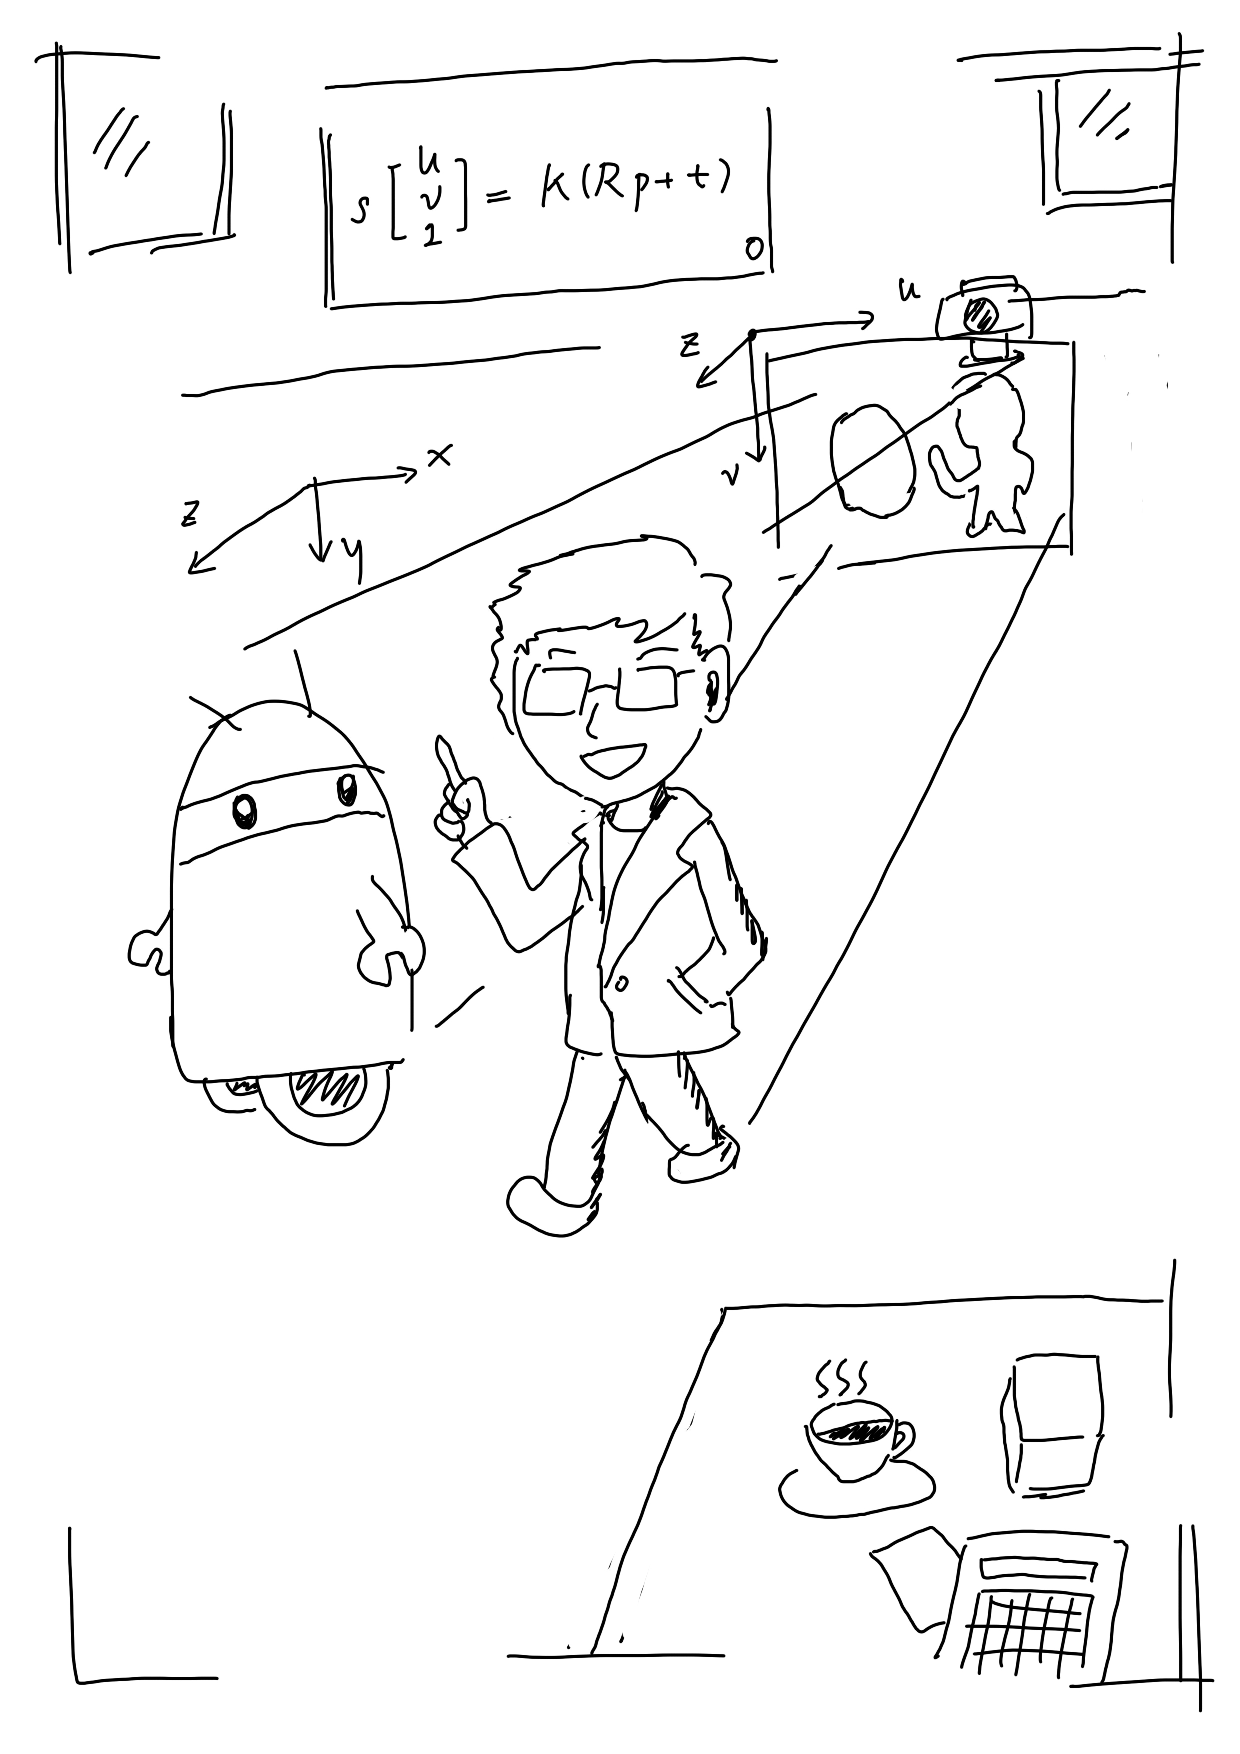
\includepdf{chapter05/resources/other/ch5.pdf}
\newpage

\section{index and logarithmic mapping}

\subsection{Basic use of Sophus}

We have introduced the introductory knowledge of Lie algebra, and now it is time to consolidate what we have learned through practical exercises. Let's discuss how to manipulate Lie algebra in a program. In Lecture 3, we saw that Eigen provided geometry modules, but did not provide support for Lie algebra. A better Lie algebra library is the Sophus library maintained by Strasdat\footnote{The earliest proposed Lie algebra is Sophus Lie, which is named after him. }. The Sophus library supports $\mathrm{SO}(3)$ and $\mathrm{SE}(3)$, which are mainly discussed in this chapter. In addition, it also contains two-dimensional motion $\mathrm{SO}(2), \mathrm{SE} (2) $ and the similar transformation of $\mathrm{Sim}(3)$. It is developed directly on top of Eigen and we don't need to install additional dependencies. Readers can get Sophus directly from GitHub, or the Sophus source code is also available in the book's code directory slambook/3rdparty. For historical reasons, earlier versions of Sophus only provided double-precision Lie group/Lie algebra classes. Subsequent versions have been rewritten as template classes. Different precision Lie group/Lie algebra can be used in the Sophus of the template class, but at the same time it increases the difficulty of use. In the second edition of this book, we use the Sophus library of \textbf{with template}. The Sophus provided in the 3rdparty of this book is the \textbf{template} version, which should have been copied when you downloaded the code for this book. Sophus itself is also a cmake project. Presumably you already know how to compile the cmake project, so I won't go into details here. The Sophus library only needs to be compiled, no need to install it.

Let's demonstrate the SO(3) and SE(3) operations in the Sophus library:

\begin{lstlisting}[language=c++,caption=slambook/ch4/useSophus.cpp]
#include <iostream>
#include <cmath>
#include <Eigen/Core>
#include <Eigen/Geometry>
#include "sophus/se3.hpp"

Using namespace std;
Using namespace Eigen;

/// This program demonstrates the basic usage of sophus
Int main(int argc, char **argv) {
// Rotation matrix rotated 90 degrees along the Z axis
Matrix3d R = AngleAxisd(M_PI / 2, Vector3d(0, 0, 1)).toRotationMatrix();
// or quaternion
Quaterniond q(R);
Sophus::SO3d SO3_R(R); // Sophus::SO3d can be constructed directly from the rotation matrix
Sophus::SO3d SO3_q(q); // can also be constructed by quaternion
// Both are equivalent
Cout << "SO(3) from matrix:\n" << SO3_R.matrix() << endl;
Cout << "SO(3) from quaternion:\n" << SO3_q.matrix() << endl;
Cout << "they are equal" << endl;

// Use the logarithmic map to get its Lie algebra
Vector3d so3 = SO3_R.log();
Cout << "so3 = " << so3.transpose() << endl;
// hat is vector to antisymmetric matrix
Cout << "so3 hat=\n" << Sophus::SO3d::hat(so3) << endl;
// Relative, vee is the objection vector
Cout << "so3 hat vee= " << Sophus::SO3d::vee(Sophus::SO3d::hat(so3)).transpose() << endl;

// Update of the incremental disturbance model
Vector3d update_so3(1e-4, 0, 0); //assuming the update is so much
Sophus::SO3d SO3_updated = Sophus::SO3d::exp(update_so3) * SO3_R;
Cout << "SO3 updated = \n" << SO3_updated.matrix() << endl;

Cout << "*******************************" << endl;
// The same is true for SE(3) operations
Vector3d t(1, 0, 0); // translate 1 along the x axis
Sophus::SE3d SE3_Rt(R, t); // Construct SE(3) from R, t
Sophus::SE3d SE3_qt(q, t); // Construct SE(3) from q,t
Cout << "SE3 from R,t= \n" << SE3_Rt.matrix() << endl;
Cout << "SE3 from q,t= \n" << SE3_qt.matrix() << endl;
// The Lie algebra se(3) is a six-dimensional vector. For convenience, typedef is used first.
Typedef Eigen::Matrix<double, 6, 1> Vector6d;
Vector6d se3 = SE3_Rt.log();
Cout << "se3 = " << se3.transpose() << endl;
// Observe the output, you will find that in Sophus, the translation of se(3) is in front and the rotation is in the back.
// Same, there are two operators of hat and vee
Cout << "se3 hat = \n" << Sophus::SE3d::hat(se3) << endl;
Cout << "se3 hat vee = " << Sophus::SE3d::vee(Sophus::SE3d::hat(se3)).transpose() << endl;

// Finally, demonstrate the update
Vector6d update_se3; //update volume
update_se3.setZero();
Update_se3(0, 0) = 1e-4d;
Sophus::SE3d SE3_updated = Sophus::SE3d::exp(update_se3) * SE3_Rt;
Cout << "SE3 updated = " << endl << SE3_updated.matrix() << endl;

Return 0;
}
\end{lstlisting}

The demo is divided into two parts. The first half introduces the operation on $\mathrm{SO}(3)$, and the second half is $\mathrm{SE}(3)$. We demonstrate how to construct $\mathrm{SO}(3), \mathrm{SE}(3)$ objects, exponentially, logarithmically map them, and update the lie group elements when we know the update amount. If the reader has a good understanding of the content of this lecture, then this program should not be difficult for you. In order to compile it, add the following lines to CMakeLists.txt:

\begin{lstlisting}[caption=slambook/ch4/useSophus/CMakeLists.txt]
# To use sophus, you need to find it using the find_package command
Find_package( Sophus REQUIRED )
Include_directories( ${Sophus_INCLUDE_DIRS} )

Add_executable( useSophus useSophus.cpp )
\end{lstlisting}

The find\_package command is an instruction provided by cmake to find the header and library files of a library. If cmake can find it, it will provide the variables for the directory where the header and library files are located. In the example of Sophus, it is Sophus\_INCLUDE\_DIRS. The template-based Sophus library, like Eigen, contains only header files and no source files. Based on them, we can introduce the Sophus library into our own cmake project. Readers are asked to see the output of this program on their own, which is consistent with our previous derivation.


\subsection{Euclidean transformation between coordinate systems}
We often define a variety of coordinate systems in the actual scene. In robotics, you define each coordinate system for each link and joint; in 3D mapping, we also define the coordinate system for each cuboid and cylinder. If you consider a moving robot, it is common practice to set an inertial coordinate system (or world coordinate system) that can be considered stationary, such as 
$ \bm{TODO(Hussein)} $ defined coordinate system. At the same time, the camera or robot is a moving coordinate system, such as the coordinate system defined by $x_C, y_C, z_C$. We might ask: a vector $\bm{p}$ in the camera's field of view, with coordinates in the camera coordinate system of $\bm{p}_c$, and in the world coordinate system, its coordinates are $ \bm{p}_w$, then how is the conversion between these two coordinates? At this time, it is necessary to first obtain the coordinate value of the point for the robot coordinate system, and then according to the robot pose \textbf{transform} into the world coordinate system. We need a mathematical means to describe this transformation. As we will see later, we can describe it with a matrix $\bm{T}$.

\begin{figure}[!htp]
	\centering
  	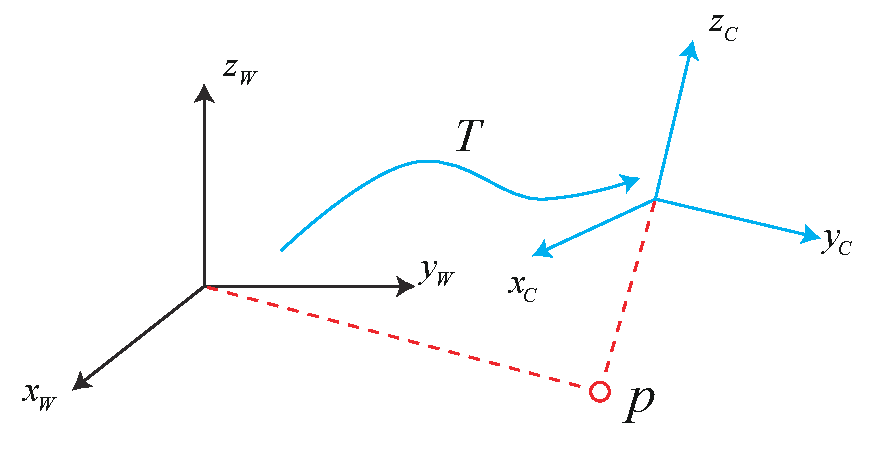
\includegraphics[width=0.7\textwidth]{chapter03/rigidMotion/axisTransform.pdf}
	\caption {Coordinate transformation. For the same vector $ \bm{} the p- $ , it coordinates in the world coordinate system $ \bm{} _w the p- $ and coordinate in the camera coordinate system $ \bm{} _c the p- $ is different. This transformation relationship is described by the transformation matrix $ \bm{T} $ . }
	\label{fig:axisTransform}
\end{figure}

Intuitively, the motion between two coordinate systems consists of a rotation plus a translation called \textbf {rigid body motion}. Camera movement is a rigid body movement. During the rigid body motion, the length and angle of the same vector in each coordinate system will not change. Imagine you throw your phone into the air and \footnote {Please don't put it into practice before it falls to the ground . }, there may only be differences in spatial position and posture, and its own length, angle of each face, etc. will not change. The phone will not be squashed like an eraser for a while, and will be stretched for a while. At this point, we say that the phone coordinate system is between the world coordinates, which is a difference of \textbf {Euclidean Transform}.

The Euclidean transformation consists of rotation and translation. We first consider rotation. Let a unit of orthogonal base $ ( \bm {e}_ 1 , \bm {e}_ 2 , \bm {e}_ 3 ) $ after a rotation becomes $ ( \bm {e}_ 1 ' , \bm {e}_ 2 ', \bm {e}_ 3 ') $ . Then, for the same vector $ \bm {a} $ (the vector does not move with the rotation of the coordinate system), its coordinates in two coordinate systems are $ [a_ 1 , a_ 2 , a_ 3 ] ^ \mathrm {T} $ and $[a'_ 1 , a'_ 2 , a'_ 3 ]^ \mathrm {T} $ . Because the vector itself has not changed, according to the definition of coordinates, there are:

\begin{equation}
\left[ \bm{e}_1,\bm{e}_2,\bm{e}_3 \right]\left[ \begin{array}{l}
{a_1}\\
{a_2}\\
{a_3}
\end{array} \right] = \left[ \bm{e}_1', \bm{e}_2', \bm{e}_3' \right]\left[ \begin{array}{l}
a'_1\\
a'_2\\
a'_3
\end{array} \right].
\end{equation}

To describe the relationship between the two coordinates, we multiply the left and right sides of the above equation by $ \left [ \begin {array}{l}
\bm{e}_1^\mathrm{T}\\
\bm{e}_2^\mathrm{T}\\
\bm{e}_3^\mathrm{T}
\end {array} \right ] $ , then the coefficient on the left becomes the identity matrix, so:
%\clearpage
\begin{equation}
\left[ \begin{array}{l}
{a_1}\\
{a_2}\\
{a_3}
\end{array}\right]=\left[{\begin{array}{*{20}{c}}    
	{\bm{e}_1^\mathrm{T}\bm{e}_1'} & {\bm{e}_1^\mathrm{T}\bm{e}_2'} & {\bm{e}_1^\mathrm{T}\bm{e}_3'}\\
	{\bm{e}_2^\mathrm{T}\bm{e}_1'} & {\bm{e}_2^\mathrm{T}\bm{e}_2'} & {\bm{e}_2^\mathrm{T}\bm{e}_3'}\\
	{\bm{e}_3^\mathrm{T}\bm{e}_1'} & {\bm{e}_3^\mathrm{T}\bm{e}_2'} & {\bm{e}_3^\mathrm{T}\bm{e}_3'}
	\end{array}} \right]\left[ \begin{array}{l}
a_1'\\
a_2'\\
a_3'
\end{array} \right] \buildrel \Delta \over = \bm{R} \bm{a}'.
\end{equation}
We take the intermediate matrix out and define it as a matrix $ \bm{R} $ . This matrix consists of the inner product between the two sets of bases, characterizing the coordinate transformation relationship of the same vector before and after the rotation. As long as the rotation is the same, then this matrix is the same. It can be said that the matrix $ \bm{R} $ describes the rotation itself. So called \textbf{rotation matrix} (Rotation matrix). At the same time, the components of the matrix are the inner product of the two coordinate system bases. Since the length of the base vector is 1, it is actually the cosine of the angle between the base vectors. So this matrix is also called \textbf{Direction Cosine Matrix}. We will call it a rotation matrix in the following.

The rotation matrix has some special properties. In fact, it is an orthogonal matrix with a determinant of 1 \footnote{orthogonal matrix that is inversely transposed by itself. The orthogonality of the rotation matrix can be derived directly from the definition. } \footnote{The determinant is 1 is artificially defined. In fact, only its determinant is $ \pm  1 $ , but the determinant is $ - 1 $ is called R rotation, that is, one rotation plus one reflection. }. Conversely, an orthogonal matrix with a determinant of 1 is also a rotation matrix. So, you can define a collection of $ n $ dimensional rotation matrices as follows:
\begin{equation}
\mathrm{SO}(n) = \{ \bm{R} \in \mathbb{R}^{n \times n} | \bm{R R}^\mathrm{T} = \bm{I}, \mathrm{det} (\bm{R})=1 \}.
\end{equation}

$ \mathrm {SO}(n) $ isthe meaningof \textbf {Special Orthogonal Group}. We leave the contents of the "group" to the next lecture. This collection consists ofa rotation matrix of $ n $ dimensional space, in particular, $ \mathrm {SO}( 3 ) $ refers to the rotation of the three-dimensional space. By rotating the matrix, we can talk directly about the rotation transformation between the two coordinate systems without having to start from the base.

Since the rotation matrix is an orthogonal matrix, its inverse (ie, transpose) describes an opposite rotation. According to the above definition, there are:
\begin{equation}
\bm{a} '= \bm{R}^{-1} \bm{a} = \bm{R}^ \mathrm{T} \bm{a}.
\end{equation}
Obviously $ \bm{R}^\mathrm{T} $ portrays an opposite rotation.

In the Euclidean transformation, there is translation in addition to rotation. Consider the vector $ \bm{a} $ in the world coordinate system , after a rotation ( depicted by $ \bm{R} $ ) and a translation of $ \bm{t} $ , you get $ \bm{a}' $ , then put the rotation and translation together, there are:
\begin{equation}
\label{eq:RT}
\ bm {a} '= \ bm {R} \ bm {a} + \ bm {t}.
\end{equation}
Where $ \bm{t} $ is called a translation vector. Compared to rotation, the translation part simply adds the translation vector to the coordinates after the rotation, which is very simple. By the above formula, we completely describe the coordinate transformation relationship of an Euclidean space using a rotation matrix $ \bm{R} $ and a translation vector $ \bm{t} $ . In practice, we will define the coordinate system 1, coordinate system 2, then the vector $ \bm{a} $ under the two coordinates is $ \bm{a}_1 , \bm{a}_2 $ , they are The relationship between the two, in accordance with the complete writing, should be:
\begin{equation}
\ bm{a}_1 = \bm{R}_{12} \bm{a}_2 + \bm{t}_{12}.
\end{equation}
Here $ \bm{R}_{12} $ means "transform the vector of coordinate system 2 into coordinate system 1". Since the vector is multiplied to the right of this matrix, its subscript is \textbf{read from right to left}. This is also the customary way of writing this book. Coordinate transformations are easy to confuse, especially if multiple coordinate systems exist. Similarly, if we want to express "rotation matrix from 1 to 2", we write it as $ \bm{R}_{21} $ . The reader must be clear about the notation here, because different books have different writing methods, some will be recorded as the top left/subscript, and the text will be written on the right side.

About panning $ \bm {t}_{12} $ , it actually corresponds to the coordinate system 1 origin pointing to the coordinate system 2 origin vector, \textbf{ coordinates taken under coordinate system}, so I suggest readers to put it It is written as "a vector from 1 to 2." But the reverse $ \bm {t}_{21} $ , which is a vector from 2 to 1 \textbf{coordinates in coordinate system 2}, is not equal to $ - \bm{t}_{12} $ , but related to the rotation of the two systems \footnote{although from the vector level, they are indeed inverse relations, but the coordinates of the two vectors are not opposite. Can you think about why this is? }. Therefore, when beginners ask the question "Where is my coordinates?", we need to clearly explain the meaning of this sentence. Here "my coordinates" actually refers to the vector from the world coordinate system pointing to the origin of the coordinate system of the world, and the coordinates obtained in the world coordinate system. Corresponding to the mathematical symbol, it should be the value of $ \bm{t}_{WC} $ . For the same reason, it is not $ - \bm {t}_{CW} $ .


\section{index and logarithmic mapping}

\subsection{Basic use of Sophus}

We have introduced the introductory knowledge of Lie algebra, and now it is time to consolidate what we have learned through practical exercises. Let's discuss how to manipulate Lie algebra in a program. In Lecture 3, we saw that Eigen provided geometry modules, but did not provide support for Lie algebra. A better Lie algebra library is the Sophus library maintained by Strasdat\footnote{The earliest proposed Lie algebra is Sophus Lie, which is named after him. }. The Sophus library supports $\mathrm{SO}(3)$ and $\mathrm{SE}(3)$, which are mainly discussed in this chapter. In addition, it also contains two-dimensional motion $\mathrm{SO}(2), \mathrm{SE} (2) $ and the similar transformation of $\mathrm{Sim}(3)$. It is developed directly on top of Eigen and we don't need to install additional dependencies. Readers can get Sophus directly from GitHub, or the Sophus source code is also available in the book's code directory slambook/3rdparty. For historical reasons, earlier versions of Sophus only provided double-precision Lie group/Lie algebra classes. Subsequent versions have been rewritten as template classes. Different precision Lie group/Lie algebra can be used in the Sophus of the template class, but at the same time it increases the difficulty of use. In the second edition of this book, we use the Sophus library of \textbf{with template}. The Sophus provided in the 3rdparty of this book is the \textbf{template} version, which should have been copied when you downloaded the code for this book. Sophus itself is also a cmake project. Presumably you already know how to compile the cmake project, so I won't go into details here. The Sophus library only needs to be compiled, no need to install it.

Let's demonstrate the SO(3) and SE(3) operations in the Sophus library:

\begin{lstlisting}[language=c++,caption=slambook/ch4/useSophus.cpp]
#include <iostream>
#include <cmath>
#include <Eigen/Core>
#include <Eigen/Geometry>
#include "sophus/se3.hpp"

Using namespace std;
Using namespace Eigen;

/// This program demonstrates the basic usage of sophus
Int main(int argc, char **argv) {
// Rotation matrix rotated 90 degrees along the Z axis
Matrix3d R = AngleAxisd(M_PI / 2, Vector3d(0, 0, 1)).toRotationMatrix();
// or quaternion
Quaterniond q(R);
Sophus::SO3d SO3_R(R); // Sophus::SO3d can be constructed directly from the rotation matrix
Sophus::SO3d SO3_q(q); // can also be constructed by quaternion
// Both are equivalent
Cout << "SO(3) from matrix:\n" << SO3_R.matrix() << endl;
Cout << "SO(3) from quaternion:\n" << SO3_q.matrix() << endl;
Cout << "they are equal" << endl;

// Use the logarithmic map to get its Lie algebra
Vector3d so3 = SO3_R.log();
Cout << "so3 = " << so3.transpose() << endl;
// hat is vector to antisymmetric matrix
Cout << "so3 hat=\n" << Sophus::SO3d::hat(so3) << endl;
// Relative, vee is the objection vector
Cout << "so3 hat vee= " << Sophus::SO3d::vee(Sophus::SO3d::hat(so3)).transpose() << endl;

// Update of the incremental disturbance model
Vector3d update_so3(1e-4, 0, 0); //assuming the update is so much
Sophus::SO3d SO3_updated = Sophus::SO3d::exp(update_so3) * SO3_R;
Cout << "SO3 updated = \n" << SO3_updated.matrix() << endl;

Cout << "*******************************" << endl;
// The same is true for SE(3) operations
Vector3d t(1, 0, 0); // translate 1 along the x axis
Sophus::SE3d SE3_Rt(R, t); // Construct SE(3) from R, t
Sophus::SE3d SE3_qt(q, t); // Construct SE(3) from q,t
Cout << "SE3 from R,t= \n" << SE3_Rt.matrix() << endl;
Cout << "SE3 from q,t= \n" << SE3_qt.matrix() << endl;
// The Lie algebra se(3) is a six-dimensional vector. For convenience, typedef is used first.
Typedef Eigen::Matrix<double, 6, 1> Vector6d;
Vector6d se3 = SE3_Rt.log();
Cout << "se3 = " << se3.transpose() << endl;
// Observe the output, you will find that in Sophus, the translation of se(3) is in front and the rotation is in the back.
// Same, there are two operators of hat and vee
Cout << "se3 hat = \n" << Sophus::SE3d::hat(se3) << endl;
Cout << "se3 hat vee = " << Sophus::SE3d::vee(Sophus::SE3d::hat(se3)).transpose() << endl;

// Finally, demonstrate the update
Vector6d update_se3; //update volume
update_se3.setZero();
Update_se3(0, 0) = 1e-4d;
Sophus::SE3d SE3_updated = Sophus::SE3d::exp(update_se3) * SE3_Rt;
Cout << "SE3 updated = " << endl << SE3_updated.matrix() << endl;

Return 0;
}
\end{lstlisting}

The demo is divided into two parts. The first half introduces the operation on $\mathrm{SO}(3)$, and the second half is $\mathrm{SE}(3)$. We demonstrate how to construct $\mathrm{SO}(3), \mathrm{SE}(3)$ objects, exponentially, logarithmically map them, and update the lie group elements when we know the update amount. If the reader has a good understanding of the content of this lecture, then this program should not be difficult for you. In order to compile it, add the following lines to CMakeLists.txt:

\begin{lstlisting}[caption=slambook/ch4/useSophus/CMakeLists.txt]
# To use sophus, you need to find it using the find_package command
Find_package( Sophus REQUIRED )
Include_directories( ${Sophus_INCLUDE_DIRS} )

Add_executable( useSophus useSophus.cpp )
\end{lstlisting}

The find\_package command is an instruction provided by cmake to find the header and library files of a library. If cmake can find it, it will provide the variables for the directory where the header and library files are located. In the example of Sophus, it is Sophus\_INCLUDE\_DIRS. The template-based Sophus library, like Eigen, contains only header files and no source files. Based on them, we can introduce the Sophus library into our own cmake project. Readers are asked to see the output of this program on their own, which is consistent with our previous derivation.


\subsection{Euclidean transformation between coordinate systems}
We often define a variety of coordinate systems in the actual scene. In robotics, you define each coordinate system for each link and joint; in 3D mapping, we also define the coordinate system for each cuboid and cylinder. If you consider a moving robot, it is common practice to set an inertial coordinate system (or world coordinate system) that can be considered stationary, such as 
$ \bm{TODO(Hussein)} $ defined coordinate system. At the same time, the camera or robot is a moving coordinate system, such as the coordinate system defined by $x_C, y_C, z_C$. We might ask: a vector $\bm{p}$ in the camera's field of view, with coordinates in the camera coordinate system of $\bm{p}_c$, and in the world coordinate system, its coordinates are $ \bm{p}_w$, then how is the conversion between these two coordinates? At this time, it is necessary to first obtain the coordinate value of the point for the robot coordinate system, and then according to the robot pose \textbf{transform} into the world coordinate system. We need a mathematical means to describe this transformation. As we will see later, we can describe it with a matrix $\bm{T}$.

\begin{figure}[!htp]
	\centering
  	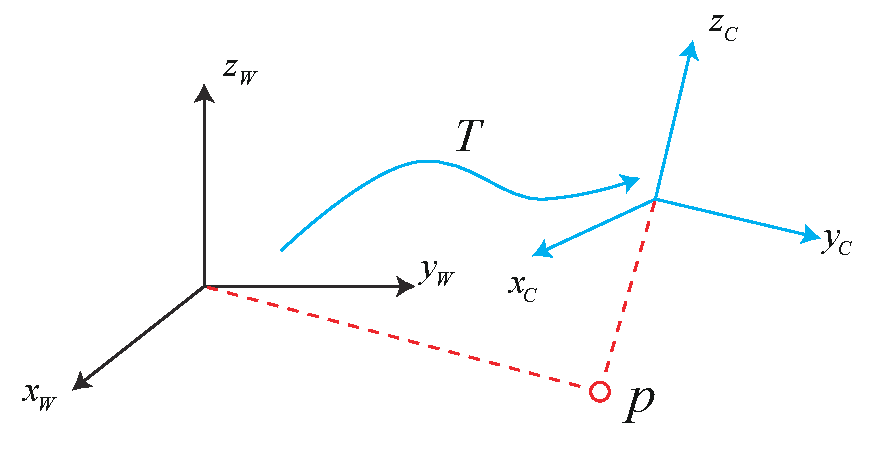
\includegraphics[width=0.7\textwidth]{chapter03/rigidMotion/axisTransform.pdf}
	\caption {Coordinate transformation. For the same vector $ \bm{} the p- $ , it coordinates in the world coordinate system $ \bm{} _w the p- $ and coordinate in the camera coordinate system $ \bm{} _c the p- $ is different. This transformation relationship is described by the transformation matrix $ \bm{T} $ . }
	\label{fig:axisTransform}
\end{figure}

Intuitively, the motion between two coordinate systems consists of a rotation plus a translation called \textbf {rigid body motion}. Camera movement is a rigid body movement. During the rigid body motion, the length and angle of the same vector in each coordinate system will not change. Imagine you throw your phone into the air and \footnote {Please don't put it into practice before it falls to the ground . }, there may only be differences in spatial position and posture, and its own length, angle of each face, etc. will not change. The phone will not be squashed like an eraser for a while, and will be stretched for a while. At this point, we say that the phone coordinate system is between the world coordinates, which is a difference of \textbf {Euclidean Transform}.

The Euclidean transformation consists of rotation and translation. We first consider rotation. Let a unit of orthogonal base $ ( \bm {e}_ 1 , \bm {e}_ 2 , \bm {e}_ 3 ) $ after a rotation becomes $ ( \bm {e}_ 1 ' , \bm {e}_ 2 ', \bm {e}_ 3 ') $ . Then, for the same vector $ \bm {a} $ (the vector does not move with the rotation of the coordinate system), its coordinates in two coordinate systems are $ [a_ 1 , a_ 2 , a_ 3 ] ^ \mathrm {T} $ and $[a'_ 1 , a'_ 2 , a'_ 3 ]^ \mathrm {T} $ . Because the vector itself has not changed, according to the definition of coordinates, there are:

\begin{equation}
\left[ \bm{e}_1,\bm{e}_2,\bm{e}_3 \right]\left[ \begin{array}{l}
{a_1}\\
{a_2}\\
{a_3}
\end{array} \right] = \left[ \bm{e}_1', \bm{e}_2', \bm{e}_3' \right]\left[ \begin{array}{l}
a'_1\\
a'_2\\
a'_3
\end{array} \right].
\end{equation}

To describe the relationship between the two coordinates, we multiply the left and right sides of the above equation by $ \left [ \begin {array}{l}
\bm{e}_1^\mathrm{T}\\
\bm{e}_2^\mathrm{T}\\
\bm{e}_3^\mathrm{T}
\end {array} \right ] $ , then the coefficient on the left becomes the identity matrix, so:
%\clearpage
\begin{equation}
\left[ \begin{array}{l}
{a_1}\\
{a_2}\\
{a_3}
\end{array}\right]=\left[{\begin{array}{*{20}{c}}    
	{\bm{e}_1^\mathrm{T}\bm{e}_1'} & {\bm{e}_1^\mathrm{T}\bm{e}_2'} & {\bm{e}_1^\mathrm{T}\bm{e}_3'}\\
	{\bm{e}_2^\mathrm{T}\bm{e}_1'} & {\bm{e}_2^\mathrm{T}\bm{e}_2'} & {\bm{e}_2^\mathrm{T}\bm{e}_3'}\\
	{\bm{e}_3^\mathrm{T}\bm{e}_1'} & {\bm{e}_3^\mathrm{T}\bm{e}_2'} & {\bm{e}_3^\mathrm{T}\bm{e}_3'}
	\end{array}} \right]\left[ \begin{array}{l}
a_1'\\
a_2'\\
a_3'
\end{array} \right] \buildrel \Delta \over = \bm{R} \bm{a}'.
\end{equation}
We take the intermediate matrix out and define it as a matrix $ \bm{R} $ . This matrix consists of the inner product between the two sets of bases, characterizing the coordinate transformation relationship of the same vector before and after the rotation. As long as the rotation is the same, then this matrix is the same. It can be said that the matrix $ \bm{R} $ describes the rotation itself. So called \textbf{rotation matrix} (Rotation matrix). At the same time, the components of the matrix are the inner product of the two coordinate system bases. Since the length of the base vector is 1, it is actually the cosine of the angle between the base vectors. So this matrix is also called \textbf{Direction Cosine Matrix}. We will call it a rotation matrix in the following.

The rotation matrix has some special properties. In fact, it is an orthogonal matrix with a determinant of 1 \footnote{orthogonal matrix that is inversely transposed by itself. The orthogonality of the rotation matrix can be derived directly from the definition. } \footnote{The determinant is 1 is artificially defined. In fact, only its determinant is $ \pm  1 $ , but the determinant is $ - 1 $ is called R rotation, that is, one rotation plus one reflection. }. Conversely, an orthogonal matrix with a determinant of 1 is also a rotation matrix. So, you can define a collection of $ n $ dimensional rotation matrices as follows:
\begin{equation}
\mathrm{SO}(n) = \{ \bm{R} \in \mathbb{R}^{n \times n} | \bm{R R}^\mathrm{T} = \bm{I}, \mathrm{det} (\bm{R})=1 \}.
\end{equation}

$ \mathrm {SO}(n) $ isthe meaningof \textbf {Special Orthogonal Group}. We leave the contents of the "group" to the next lecture. This collection consists ofa rotation matrix of $ n $ dimensional space, in particular, $ \mathrm {SO}( 3 ) $ refers to the rotation of the three-dimensional space. By rotating the matrix, we can talk directly about the rotation transformation between the two coordinate systems without having to start from the base.

Since the rotation matrix is an orthogonal matrix, its inverse (ie, transpose) describes an opposite rotation. According to the above definition, there are:
\begin{equation}
\bm{a} '= \bm{R}^{-1} \bm{a} = \bm{R}^ \mathrm{T} \bm{a}.
\end{equation}
Obviously $ \bm{R}^\mathrm{T} $ portrays an opposite rotation.

In the Euclidean transformation, there is translation in addition to rotation. Consider the vector $ \bm{a} $ in the world coordinate system , after a rotation ( depicted by $ \bm{R} $ ) and a translation of $ \bm{t} $ , you get $ \bm{a}' $ , then put the rotation and translation together, there are:
\begin{equation}
\label{eq:RT}
\ bm {a} '= \ bm {R} \ bm {a} + \ bm {t}.
\end{equation}
Where $ \bm{t} $ is called a translation vector. Compared to rotation, the translation part simply adds the translation vector to the coordinates after the rotation, which is very simple. By the above formula, we completely describe the coordinate transformation relationship of an Euclidean space using a rotation matrix $ \bm{R} $ and a translation vector $ \bm{t} $ . In practice, we will define the coordinate system 1, coordinate system 2, then the vector $ \bm{a} $ under the two coordinates is $ \bm{a}_1 , \bm{a}_2 $ , they are The relationship between the two, in accordance with the complete writing, should be:
\begin{equation}
\ bm{a}_1 = \bm{R}_{12} \bm{a}_2 + \bm{t}_{12}.
\end{equation}
Here $ \bm{R}_{12} $ means "transform the vector of coordinate system 2 into coordinate system 1". Since the vector is multiplied to the right of this matrix, its subscript is \textbf{read from right to left}. This is also the customary way of writing this book. Coordinate transformations are easy to confuse, especially if multiple coordinate systems exist. Similarly, if we want to express "rotation matrix from 1 to 2", we write it as $ \bm{R}_{21} $ . The reader must be clear about the notation here, because different books have different writing methods, some will be recorded as the top left/subscript, and the text will be written on the right side.

About panning $ \bm {t}_{12} $ , it actually corresponds to the coordinate system 1 origin pointing to the coordinate system 2 origin vector, \textbf{ coordinates taken under coordinate system}, so I suggest readers to put it It is written as "a vector from 1 to 2." But the reverse $ \bm {t}_{21} $ , which is a vector from 2 to 1 \textbf{coordinates in coordinate system 2}, is not equal to $ - \bm{t}_{12} $ , but related to the rotation of the two systems \footnote{although from the vector level, they are indeed inverse relations, but the coordinates of the two vectors are not opposite. Can you think about why this is? }. Therefore, when beginners ask the question "Where is my coordinates?", we need to clearly explain the meaning of this sentence. Here "my coordinates" actually refers to the vector from the world coordinate system pointing to the origin of the coordinate system of the world, and the coordinates obtained in the world coordinate system. Corresponding to the mathematical symbol, it should be the value of $ \bm{t}_{WC} $ . For the same reason, it is not $ - \bm {t}_{CW} $ .


\section{index and logarithmic mapping}

\subsection{Basic use of Sophus}

We have introduced the introductory knowledge of Lie algebra, and now it is time to consolidate what we have learned through practical exercises. Let's discuss how to manipulate Lie algebra in a program. In Lecture 3, we saw that Eigen provided geometry modules, but did not provide support for Lie algebra. A better Lie algebra library is the Sophus library maintained by Strasdat\footnote{The earliest proposed Lie algebra is Sophus Lie, which is named after him. }. The Sophus library supports $\mathrm{SO}(3)$ and $\mathrm{SE}(3)$, which are mainly discussed in this chapter. In addition, it also contains two-dimensional motion $\mathrm{SO}(2), \mathrm{SE} (2) $ and the similar transformation of $\mathrm{Sim}(3)$. It is developed directly on top of Eigen and we don't need to install additional dependencies. Readers can get Sophus directly from GitHub, or the Sophus source code is also available in the book's code directory slambook/3rdparty. For historical reasons, earlier versions of Sophus only provided double-precision Lie group/Lie algebra classes. Subsequent versions have been rewritten as template classes. Different precision Lie group/Lie algebra can be used in the Sophus of the template class, but at the same time it increases the difficulty of use. In the second edition of this book, we use the Sophus library of \textbf{with template}. The Sophus provided in the 3rdparty of this book is the \textbf{template} version, which should have been copied when you downloaded the code for this book. Sophus itself is also a cmake project. Presumably you already know how to compile the cmake project, so I won't go into details here. The Sophus library only needs to be compiled, no need to install it.

Let's demonstrate the SO(3) and SE(3) operations in the Sophus library:

\begin{lstlisting}[language=c++,caption=slambook/ch4/useSophus.cpp]
#include <iostream>
#include <cmath>
#include <Eigen/Core>
#include <Eigen/Geometry>
#include "sophus/se3.hpp"

Using namespace std;
Using namespace Eigen;

/// This program demonstrates the basic usage of sophus
Int main(int argc, char **argv) {
// Rotation matrix rotated 90 degrees along the Z axis
Matrix3d R = AngleAxisd(M_PI / 2, Vector3d(0, 0, 1)).toRotationMatrix();
// or quaternion
Quaterniond q(R);
Sophus::SO3d SO3_R(R); // Sophus::SO3d can be constructed directly from the rotation matrix
Sophus::SO3d SO3_q(q); // can also be constructed by quaternion
// Both are equivalent
Cout << "SO(3) from matrix:\n" << SO3_R.matrix() << endl;
Cout << "SO(3) from quaternion:\n" << SO3_q.matrix() << endl;
Cout << "they are equal" << endl;

// Use the logarithmic map to get its Lie algebra
Vector3d so3 = SO3_R.log();
Cout << "so3 = " << so3.transpose() << endl;
// hat is vector to antisymmetric matrix
Cout << "so3 hat=\n" << Sophus::SO3d::hat(so3) << endl;
// Relative, vee is the objection vector
Cout << "so3 hat vee= " << Sophus::SO3d::vee(Sophus::SO3d::hat(so3)).transpose() << endl;

// Update of the incremental disturbance model
Vector3d update_so3(1e-4, 0, 0); //assuming the update is so much
Sophus::SO3d SO3_updated = Sophus::SO3d::exp(update_so3) * SO3_R;
Cout << "SO3 updated = \n" << SO3_updated.matrix() << endl;

Cout << "*******************************" << endl;
// The same is true for SE(3) operations
Vector3d t(1, 0, 0); // translate 1 along the x axis
Sophus::SE3d SE3_Rt(R, t); // Construct SE(3) from R, t
Sophus::SE3d SE3_qt(q, t); // Construct SE(3) from q,t
Cout << "SE3 from R,t= \n" << SE3_Rt.matrix() << endl;
Cout << "SE3 from q,t= \n" << SE3_qt.matrix() << endl;
// The Lie algebra se(3) is a six-dimensional vector. For convenience, typedef is used first.
Typedef Eigen::Matrix<double, 6, 1> Vector6d;
Vector6d se3 = SE3_Rt.log();
Cout << "se3 = " << se3.transpose() << endl;
// Observe the output, you will find that in Sophus, the translation of se(3) is in front and the rotation is in the back.
// Same, there are two operators of hat and vee
Cout << "se3 hat = \n" << Sophus::SE3d::hat(se3) << endl;
Cout << "se3 hat vee = " << Sophus::SE3d::vee(Sophus::SE3d::hat(se3)).transpose() << endl;

// Finally, demonstrate the update
Vector6d update_se3; //update volume
update_se3.setZero();
Update_se3(0, 0) = 1e-4d;
Sophus::SE3d SE3_updated = Sophus::SE3d::exp(update_se3) * SE3_Rt;
Cout << "SE3 updated = " << endl << SE3_updated.matrix() << endl;

Return 0;
}
\end{lstlisting}

The demo is divided into two parts. The first half introduces the operation on $\mathrm{SO}(3)$, and the second half is $\mathrm{SE}(3)$. We demonstrate how to construct $\mathrm{SO}(3), \mathrm{SE}(3)$ objects, exponentially, logarithmically map them, and update the lie group elements when we know the update amount. If the reader has a good understanding of the content of this lecture, then this program should not be difficult for you. In order to compile it, add the following lines to CMakeLists.txt:

\begin{lstlisting}[caption=slambook/ch4/useSophus/CMakeLists.txt]
# To use sophus, you need to find it using the find_package command
Find_package( Sophus REQUIRED )
Include_directories( ${Sophus_INCLUDE_DIRS} )

Add_executable( useSophus useSophus.cpp )
\end{lstlisting}

The find\_package command is an instruction provided by cmake to find the header and library files of a library. If cmake can find it, it will provide the variables for the directory where the header and library files are located. In the example of Sophus, it is Sophus\_INCLUDE\_DIRS. The template-based Sophus library, like Eigen, contains only header files and no source files. Based on them, we can introduce the Sophus library into our own cmake project. Readers are asked to see the output of this program on their own, which is consistent with our previous derivation.


\subsection{Euclidean transformation between coordinate systems}
We often define a variety of coordinate systems in the actual scene. In robotics, you define each coordinate system for each link and joint; in 3D mapping, we also define the coordinate system for each cuboid and cylinder. If you consider a moving robot, it is common practice to set an inertial coordinate system (or world coordinate system) that can be considered stationary, such as 
$ \bm{TODO(Hussein)} $ defined coordinate system. At the same time, the camera or robot is a moving coordinate system, such as the coordinate system defined by $x_C, y_C, z_C$. We might ask: a vector $\bm{p}$ in the camera's field of view, with coordinates in the camera coordinate system of $\bm{p}_c$, and in the world coordinate system, its coordinates are $ \bm{p}_w$, then how is the conversion between these two coordinates? At this time, it is necessary to first obtain the coordinate value of the point for the robot coordinate system, and then according to the robot pose \textbf{transform} into the world coordinate system. We need a mathematical means to describe this transformation. As we will see later, we can describe it with a matrix $\bm{T}$.

\begin{figure}[!htp]
	\centering
  	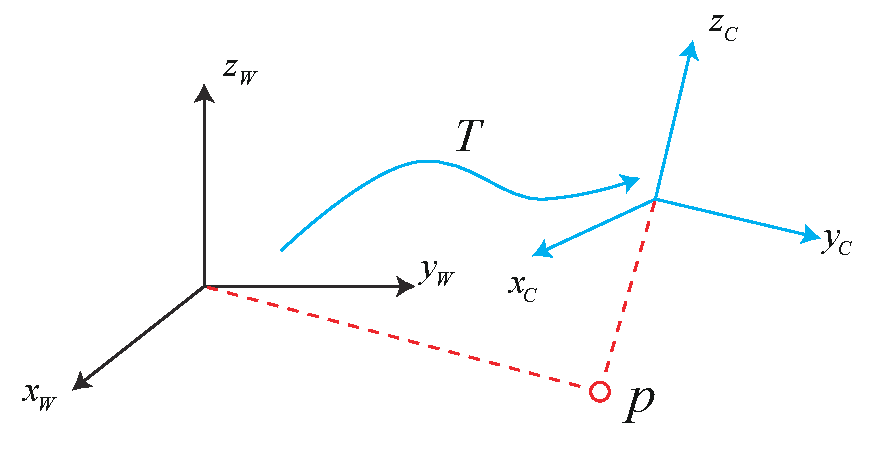
\includegraphics[width=0.7\textwidth]{chapter03/rigidMotion/axisTransform.pdf}
	\caption {Coordinate transformation. For the same vector $ \bm{} the p- $ , it coordinates in the world coordinate system $ \bm{} _w the p- $ and coordinate in the camera coordinate system $ \bm{} _c the p- $ is different. This transformation relationship is described by the transformation matrix $ \bm{T} $ . }
	\label{fig:axisTransform}
\end{figure}

Intuitively, the motion between two coordinate systems consists of a rotation plus a translation called \textbf {rigid body motion}. Camera movement is a rigid body movement. During the rigid body motion, the length and angle of the same vector in each coordinate system will not change. Imagine you throw your phone into the air and \footnote {Please don't put it into practice before it falls to the ground . }, there may only be differences in spatial position and posture, and its own length, angle of each face, etc. will not change. The phone will not be squashed like an eraser for a while, and will be stretched for a while. At this point, we say that the phone coordinate system is between the world coordinates, which is a difference of \textbf {Euclidean Transform}.

The Euclidean transformation consists of rotation and translation. We first consider rotation. Let a unit of orthogonal base $ ( \bm {e}_ 1 , \bm {e}_ 2 , \bm {e}_ 3 ) $ after a rotation becomes $ ( \bm {e}_ 1 ' , \bm {e}_ 2 ', \bm {e}_ 3 ') $ . Then, for the same vector $ \bm {a} $ (the vector does not move with the rotation of the coordinate system), its coordinates in two coordinate systems are $ [a_ 1 , a_ 2 , a_ 3 ] ^ \mathrm {T} $ and $[a'_ 1 , a'_ 2 , a'_ 3 ]^ \mathrm {T} $ . Because the vector itself has not changed, according to the definition of coordinates, there are:

\begin{equation}
\left[ \bm{e}_1,\bm{e}_2,\bm{e}_3 \right]\left[ \begin{array}{l}
{a_1}\\
{a_2}\\
{a_3}
\end{array} \right] = \left[ \bm{e}_1', \bm{e}_2', \bm{e}_3' \right]\left[ \begin{array}{l}
a'_1\\
a'_2\\
a'_3
\end{array} \right].
\end{equation}

To describe the relationship between the two coordinates, we multiply the left and right sides of the above equation by $ \left [ \begin {array}{l}
\bm{e}_1^\mathrm{T}\\
\bm{e}_2^\mathrm{T}\\
\bm{e}_3^\mathrm{T}
\end {array} \right ] $ , then the coefficient on the left becomes the identity matrix, so:
%\clearpage
\begin{equation}
\left[ \begin{array}{l}
{a_1}\\
{a_2}\\
{a_3}
\end{array}\right]=\left[{\begin{array}{*{20}{c}}    
	{\bm{e}_1^\mathrm{T}\bm{e}_1'} & {\bm{e}_1^\mathrm{T}\bm{e}_2'} & {\bm{e}_1^\mathrm{T}\bm{e}_3'}\\
	{\bm{e}_2^\mathrm{T}\bm{e}_1'} & {\bm{e}_2^\mathrm{T}\bm{e}_2'} & {\bm{e}_2^\mathrm{T}\bm{e}_3'}\\
	{\bm{e}_3^\mathrm{T}\bm{e}_1'} & {\bm{e}_3^\mathrm{T}\bm{e}_2'} & {\bm{e}_3^\mathrm{T}\bm{e}_3'}
	\end{array}} \right]\left[ \begin{array}{l}
a_1'\\
a_2'\\
a_3'
\end{array} \right] \buildrel \Delta \over = \bm{R} \bm{a}'.
\end{equation}
We take the intermediate matrix out and define it as a matrix $ \bm{R} $ . This matrix consists of the inner product between the two sets of bases, characterizing the coordinate transformation relationship of the same vector before and after the rotation. As long as the rotation is the same, then this matrix is the same. It can be said that the matrix $ \bm{R} $ describes the rotation itself. So called \textbf{rotation matrix} (Rotation matrix). At the same time, the components of the matrix are the inner product of the two coordinate system bases. Since the length of the base vector is 1, it is actually the cosine of the angle between the base vectors. So this matrix is also called \textbf{Direction Cosine Matrix}. We will call it a rotation matrix in the following.

The rotation matrix has some special properties. In fact, it is an orthogonal matrix with a determinant of 1 \footnote{orthogonal matrix that is inversely transposed by itself. The orthogonality of the rotation matrix can be derived directly from the definition. } \footnote{The determinant is 1 is artificially defined. In fact, only its determinant is $ \pm  1 $ , but the determinant is $ - 1 $ is called R rotation, that is, one rotation plus one reflection. }. Conversely, an orthogonal matrix with a determinant of 1 is also a rotation matrix. So, you can define a collection of $ n $ dimensional rotation matrices as follows:
\begin{equation}
\mathrm{SO}(n) = \{ \bm{R} \in \mathbb{R}^{n \times n} | \bm{R R}^\mathrm{T} = \bm{I}, \mathrm{det} (\bm{R})=1 \}.
\end{equation}

$ \mathrm {SO}(n) $ isthe meaningof \textbf {Special Orthogonal Group}. We leave the contents of the "group" to the next lecture. This collection consists ofa rotation matrix of $ n $ dimensional space, in particular, $ \mathrm {SO}( 3 ) $ refers to the rotation of the three-dimensional space. By rotating the matrix, we can talk directly about the rotation transformation between the two coordinate systems without having to start from the base.

Since the rotation matrix is an orthogonal matrix, its inverse (ie, transpose) describes an opposite rotation. According to the above definition, there are:
\begin{equation}
\bm{a} '= \bm{R}^{-1} \bm{a} = \bm{R}^ \mathrm{T} \bm{a}.
\end{equation}
Obviously $ \bm{R}^\mathrm{T} $ portrays an opposite rotation.

In the Euclidean transformation, there is translation in addition to rotation. Consider the vector $ \bm{a} $ in the world coordinate system , after a rotation ( depicted by $ \bm{R} $ ) and a translation of $ \bm{t} $ , you get $ \bm{a}' $ , then put the rotation and translation together, there are:
\begin{equation}
\label{eq:RT}
\ bm {a} '= \ bm {R} \ bm {a} + \ bm {t}.
\end{equation}
Where $ \bm{t} $ is called a translation vector. Compared to rotation, the translation part simply adds the translation vector to the coordinates after the rotation, which is very simple. By the above formula, we completely describe the coordinate transformation relationship of an Euclidean space using a rotation matrix $ \bm{R} $ and a translation vector $ \bm{t} $ . In practice, we will define the coordinate system 1, coordinate system 2, then the vector $ \bm{a} $ under the two coordinates is $ \bm{a}_1 , \bm{a}_2 $ , they are The relationship between the two, in accordance with the complete writing, should be:
\begin{equation}
\ bm{a}_1 = \bm{R}_{12} \bm{a}_2 + \bm{t}_{12}.
\end{equation}
Here $ \bm{R}_{12} $ means "transform the vector of coordinate system 2 into coordinate system 1". Since the vector is multiplied to the right of this matrix, its subscript is \textbf{read from right to left}. This is also the customary way of writing this book. Coordinate transformations are easy to confuse, especially if multiple coordinate systems exist. Similarly, if we want to express "rotation matrix from 1 to 2", we write it as $ \bm{R}_{21} $ . The reader must be clear about the notation here, because different books have different writing methods, some will be recorded as the top left/subscript, and the text will be written on the right side.

About panning $ \bm {t}_{12} $ , it actually corresponds to the coordinate system 1 origin pointing to the coordinate system 2 origin vector, \textbf{ coordinates taken under coordinate system}, so I suggest readers to put it It is written as "a vector from 1 to 2." But the reverse $ \bm {t}_{21} $ , which is a vector from 2 to 1 \textbf{coordinates in coordinate system 2}, is not equal to $ - \bm{t}_{12} $ , but related to the rotation of the two systems \footnote{although from the vector level, they are indeed inverse relations, but the coordinates of the two vectors are not opposite. Can you think about why this is? }. Therefore, when beginners ask the question "Where is my coordinates?", we need to clearly explain the meaning of this sentence. Here "my coordinates" actually refers to the vector from the world coordinate system pointing to the origin of the coordinate system of the world, and the coordinates obtained in the world coordinate system. Corresponding to the mathematical symbol, it should be the value of $ \bm{t}_{WC} $ . For the same reason, it is not $ - \bm {t}_{CW} $ .


\section{index and logarithmic mapping}

\subsection{Basic use of Sophus}

We have introduced the introductory knowledge of Lie algebra, and now it is time to consolidate what we have learned through practical exercises. Let's discuss how to manipulate Lie algebra in a program. In Lecture 3, we saw that Eigen provided geometry modules, but did not provide support for Lie algebra. A better Lie algebra library is the Sophus library maintained by Strasdat\footnote{The earliest proposed Lie algebra is Sophus Lie, which is named after him. }. The Sophus library supports $\mathrm{SO}(3)$ and $\mathrm{SE}(3)$, which are mainly discussed in this chapter. In addition, it also contains two-dimensional motion $\mathrm{SO}(2), \mathrm{SE} (2) $ and the similar transformation of $\mathrm{Sim}(3)$. It is developed directly on top of Eigen and we don't need to install additional dependencies. Readers can get Sophus directly from GitHub, or the Sophus source code is also available in the book's code directory slambook/3rdparty. For historical reasons, earlier versions of Sophus only provided double-precision Lie group/Lie algebra classes. Subsequent versions have been rewritten as template classes. Different precision Lie group/Lie algebra can be used in the Sophus of the template class, but at the same time it increases the difficulty of use. In the second edition of this book, we use the Sophus library of \textbf{with template}. The Sophus provided in the 3rdparty of this book is the \textbf{template} version, which should have been copied when you downloaded the code for this book. Sophus itself is also a cmake project. Presumably you already know how to compile the cmake project, so I won't go into details here. The Sophus library only needs to be compiled, no need to install it.

Let's demonstrate the SO(3) and SE(3) operations in the Sophus library:

\begin{lstlisting}[language=c++,caption=slambook/ch4/useSophus.cpp]
#include <iostream>
#include <cmath>
#include <Eigen/Core>
#include <Eigen/Geometry>
#include "sophus/se3.hpp"

Using namespace std;
Using namespace Eigen;

/// This program demonstrates the basic usage of sophus
Int main(int argc, char **argv) {
// Rotation matrix rotated 90 degrees along the Z axis
Matrix3d R = AngleAxisd(M_PI / 2, Vector3d(0, 0, 1)).toRotationMatrix();
// or quaternion
Quaterniond q(R);
Sophus::SO3d SO3_R(R); // Sophus::SO3d can be constructed directly from the rotation matrix
Sophus::SO3d SO3_q(q); // can also be constructed by quaternion
// Both are equivalent
Cout << "SO(3) from matrix:\n" << SO3_R.matrix() << endl;
Cout << "SO(3) from quaternion:\n" << SO3_q.matrix() << endl;
Cout << "they are equal" << endl;

// Use the logarithmic map to get its Lie algebra
Vector3d so3 = SO3_R.log();
Cout << "so3 = " << so3.transpose() << endl;
// hat is vector to antisymmetric matrix
Cout << "so3 hat=\n" << Sophus::SO3d::hat(so3) << endl;
// Relative, vee is the objection vector
Cout << "so3 hat vee= " << Sophus::SO3d::vee(Sophus::SO3d::hat(so3)).transpose() << endl;

// Update of the incremental disturbance model
Vector3d update_so3(1e-4, 0, 0); //assuming the update is so much
Sophus::SO3d SO3_updated = Sophus::SO3d::exp(update_so3) * SO3_R;
Cout << "SO3 updated = \n" << SO3_updated.matrix() << endl;

Cout << "*******************************" << endl;
// The same is true for SE(3) operations
Vector3d t(1, 0, 0); // translate 1 along the x axis
Sophus::SE3d SE3_Rt(R, t); // Construct SE(3) from R, t
Sophus::SE3d SE3_qt(q, t); // Construct SE(3) from q,t
Cout << "SE3 from R,t= \n" << SE3_Rt.matrix() << endl;
Cout << "SE3 from q,t= \n" << SE3_qt.matrix() << endl;
// The Lie algebra se(3) is a six-dimensional vector. For convenience, typedef is used first.
Typedef Eigen::Matrix<double, 6, 1> Vector6d;
Vector6d se3 = SE3_Rt.log();
Cout << "se3 = " << se3.transpose() << endl;
// Observe the output, you will find that in Sophus, the translation of se(3) is in front and the rotation is in the back.
// Same, there are two operators of hat and vee
Cout << "se3 hat = \n" << Sophus::SE3d::hat(se3) << endl;
Cout << "se3 hat vee = " << Sophus::SE3d::vee(Sophus::SE3d::hat(se3)).transpose() << endl;

// Finally, demonstrate the update
Vector6d update_se3; //update volume
update_se3.setZero();
Update_se3(0, 0) = 1e-4d;
Sophus::SE3d SE3_updated = Sophus::SE3d::exp(update_se3) * SE3_Rt;
Cout << "SE3 updated = " << endl << SE3_updated.matrix() << endl;

Return 0;
}
\end{lstlisting}

The demo is divided into two parts. The first half introduces the operation on $\mathrm{SO}(3)$, and the second half is $\mathrm{SE}(3)$. We demonstrate how to construct $\mathrm{SO}(3), \mathrm{SE}(3)$ objects, exponentially, logarithmically map them, and update the lie group elements when we know the update amount. If the reader has a good understanding of the content of this lecture, then this program should not be difficult for you. In order to compile it, add the following lines to CMakeLists.txt:

\begin{lstlisting}[caption=slambook/ch4/useSophus/CMakeLists.txt]
# To use sophus, you need to find it using the find_package command
Find_package( Sophus REQUIRED )
Include_directories( ${Sophus_INCLUDE_DIRS} )

Add_executable( useSophus useSophus.cpp )
\end{lstlisting}

The find\_package command is an instruction provided by cmake to find the header and library files of a library. If cmake can find it, it will provide the variables for the directory where the header and library files are located. In the example of Sophus, it is Sophus\_INCLUDE\_DIRS. The template-based Sophus library, like Eigen, contains only header files and no source files. Based on them, we can introduce the Sophus library into our own cmake project. Readers are asked to see the output of this program on their own, which is consistent with our previous derivation.


\subsection{Euclidean transformation between coordinate systems}
We often define a variety of coordinate systems in the actual scene. In robotics, you define each coordinate system for each link and joint; in 3D mapping, we also define the coordinate system for each cuboid and cylinder. If you consider a moving robot, it is common practice to set an inertial coordinate system (or world coordinate system) that can be considered stationary, such as 
$ \bm{TODO(Hussein)} $ defined coordinate system. At the same time, the camera or robot is a moving coordinate system, such as the coordinate system defined by $x_C, y_C, z_C$. We might ask: a vector $\bm{p}$ in the camera's field of view, with coordinates in the camera coordinate system of $\bm{p}_c$, and in the world coordinate system, its coordinates are $ \bm{p}_w$, then how is the conversion between these two coordinates? At this time, it is necessary to first obtain the coordinate value of the point for the robot coordinate system, and then according to the robot pose \textbf{transform} into the world coordinate system. We need a mathematical means to describe this transformation. As we will see later, we can describe it with a matrix $\bm{T}$.

\begin{figure}[!htp]
	\centering
  	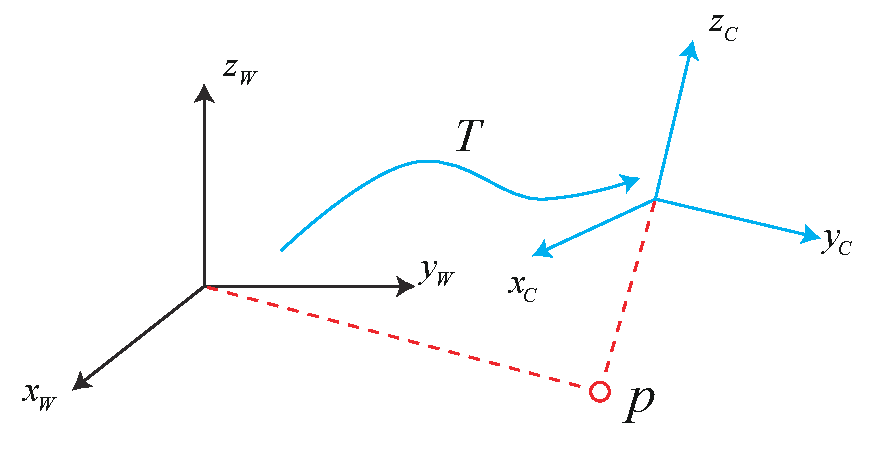
\includegraphics[width=0.7\textwidth]{chapter03/rigidMotion/axisTransform.pdf}
	\caption {Coordinate transformation. For the same vector $ \bm{} the p- $ , it coordinates in the world coordinate system $ \bm{} _w the p- $ and coordinate in the camera coordinate system $ \bm{} _c the p- $ is different. This transformation relationship is described by the transformation matrix $ \bm{T} $ . }
	\label{fig:axisTransform}
\end{figure}

Intuitively, the motion between two coordinate systems consists of a rotation plus a translation called \textbf {rigid body motion}. Camera movement is a rigid body movement. During the rigid body motion, the length and angle of the same vector in each coordinate system will not change. Imagine you throw your phone into the air and \footnote {Please don't put it into practice before it falls to the ground . }, there may only be differences in spatial position and posture, and its own length, angle of each face, etc. will not change. The phone will not be squashed like an eraser for a while, and will be stretched for a while. At this point, we say that the phone coordinate system is between the world coordinates, which is a difference of \textbf {Euclidean Transform}.

The Euclidean transformation consists of rotation and translation. We first consider rotation. Let a unit of orthogonal base $ ( \bm {e}_ 1 , \bm {e}_ 2 , \bm {e}_ 3 ) $ after a rotation becomes $ ( \bm {e}_ 1 ' , \bm {e}_ 2 ', \bm {e}_ 3 ') $ . Then, for the same vector $ \bm {a} $ (the vector does not move with the rotation of the coordinate system), its coordinates in two coordinate systems are $ [a_ 1 , a_ 2 , a_ 3 ] ^ \mathrm {T} $ and $[a'_ 1 , a'_ 2 , a'_ 3 ]^ \mathrm {T} $ . Because the vector itself has not changed, according to the definition of coordinates, there are:

\begin{equation}
\left[ \bm{e}_1,\bm{e}_2,\bm{e}_3 \right]\left[ \begin{array}{l}
{a_1}\\
{a_2}\\
{a_3}
\end{array} \right] = \left[ \bm{e}_1', \bm{e}_2', \bm{e}_3' \right]\left[ \begin{array}{l}
a'_1\\
a'_2\\
a'_3
\end{array} \right].
\end{equation}

To describe the relationship between the two coordinates, we multiply the left and right sides of the above equation by $ \left [ \begin {array}{l}
\bm{e}_1^\mathrm{T}\\
\bm{e}_2^\mathrm{T}\\
\bm{e}_3^\mathrm{T}
\end {array} \right ] $ , then the coefficient on the left becomes the identity matrix, so:
%\clearpage
\begin{equation}
\left[ \begin{array}{l}
{a_1}\\
{a_2}\\
{a_3}
\end{array}\right]=\left[{\begin{array}{*{20}{c}}    
	{\bm{e}_1^\mathrm{T}\bm{e}_1'} & {\bm{e}_1^\mathrm{T}\bm{e}_2'} & {\bm{e}_1^\mathrm{T}\bm{e}_3'}\\
	{\bm{e}_2^\mathrm{T}\bm{e}_1'} & {\bm{e}_2^\mathrm{T}\bm{e}_2'} & {\bm{e}_2^\mathrm{T}\bm{e}_3'}\\
	{\bm{e}_3^\mathrm{T}\bm{e}_1'} & {\bm{e}_3^\mathrm{T}\bm{e}_2'} & {\bm{e}_3^\mathrm{T}\bm{e}_3'}
	\end{array}} \right]\left[ \begin{array}{l}
a_1'\\
a_2'\\
a_3'
\end{array} \right] \buildrel \Delta \over = \bm{R} \bm{a}'.
\end{equation}
We take the intermediate matrix out and define it as a matrix $ \bm{R} $ . This matrix consists of the inner product between the two sets of bases, characterizing the coordinate transformation relationship of the same vector before and after the rotation. As long as the rotation is the same, then this matrix is the same. It can be said that the matrix $ \bm{R} $ describes the rotation itself. So called \textbf{rotation matrix} (Rotation matrix). At the same time, the components of the matrix are the inner product of the two coordinate system bases. Since the length of the base vector is 1, it is actually the cosine of the angle between the base vectors. So this matrix is also called \textbf{Direction Cosine Matrix}. We will call it a rotation matrix in the following.

The rotation matrix has some special properties. In fact, it is an orthogonal matrix with a determinant of 1 \footnote{orthogonal matrix that is inversely transposed by itself. The orthogonality of the rotation matrix can be derived directly from the definition. } \footnote{The determinant is 1 is artificially defined. In fact, only its determinant is $ \pm  1 $ , but the determinant is $ - 1 $ is called R rotation, that is, one rotation plus one reflection. }. Conversely, an orthogonal matrix with a determinant of 1 is also a rotation matrix. So, you can define a collection of $ n $ dimensional rotation matrices as follows:
\begin{equation}
\mathrm{SO}(n) = \{ \bm{R} \in \mathbb{R}^{n \times n} | \bm{R R}^\mathrm{T} = \bm{I}, \mathrm{det} (\bm{R})=1 \}.
\end{equation}

$ \mathrm {SO}(n) $ isthe meaningof \textbf {Special Orthogonal Group}. We leave the contents of the "group" to the next lecture. This collection consists ofa rotation matrix of $ n $ dimensional space, in particular, $ \mathrm {SO}( 3 ) $ refers to the rotation of the three-dimensional space. By rotating the matrix, we can talk directly about the rotation transformation between the two coordinate systems without having to start from the base.

Since the rotation matrix is an orthogonal matrix, its inverse (ie, transpose) describes an opposite rotation. According to the above definition, there are:
\begin{equation}
\bm{a} '= \bm{R}^{-1} \bm{a} = \bm{R}^ \mathrm{T} \bm{a}.
\end{equation}
Obviously $ \bm{R}^\mathrm{T} $ portrays an opposite rotation.

In the Euclidean transformation, there is translation in addition to rotation. Consider the vector $ \bm{a} $ in the world coordinate system , after a rotation ( depicted by $ \bm{R} $ ) and a translation of $ \bm{t} $ , you get $ \bm{a}' $ , then put the rotation and translation together, there are:
\begin{equation}
\label{eq:RT}
\ bm {a} '= \ bm {R} \ bm {a} + \ bm {t}.
\end{equation}
Where $ \bm{t} $ is called a translation vector. Compared to rotation, the translation part simply adds the translation vector to the coordinates after the rotation, which is very simple. By the above formula, we completely describe the coordinate transformation relationship of an Euclidean space using a rotation matrix $ \bm{R} $ and a translation vector $ \bm{t} $ . In practice, we will define the coordinate system 1, coordinate system 2, then the vector $ \bm{a} $ under the two coordinates is $ \bm{a}_1 , \bm{a}_2 $ , they are The relationship between the two, in accordance with the complete writing, should be:
\begin{equation}
\ bm{a}_1 = \bm{R}_{12} \bm{a}_2 + \bm{t}_{12}.
\end{equation}
Here $ \bm{R}_{12} $ means "transform the vector of coordinate system 2 into coordinate system 1". Since the vector is multiplied to the right of this matrix, its subscript is \textbf{read from right to left}. This is also the customary way of writing this book. Coordinate transformations are easy to confuse, especially if multiple coordinate systems exist. Similarly, if we want to express "rotation matrix from 1 to 2", we write it as $ \bm{R}_{21} $ . The reader must be clear about the notation here, because different books have different writing methods, some will be recorded as the top left/subscript, and the text will be written on the right side.

About panning $ \bm {t}_{12} $ , it actually corresponds to the coordinate system 1 origin pointing to the coordinate system 2 origin vector, \textbf{ coordinates taken under coordinate system}, so I suggest readers to put it It is written as "a vector from 1 to 2." But the reverse $ \bm {t}_{21} $ , which is a vector from 2 to 1 \textbf{coordinates in coordinate system 2}, is not equal to $ - \bm{t}_{12} $ , but related to the rotation of the two systems \footnote{although from the vector level, they are indeed inverse relations, but the coordinates of the two vectors are not opposite. Can you think about why this is? }. Therefore, when beginners ask the question "Where is my coordinates?", we need to clearly explain the meaning of this sentence. Here "my coordinates" actually refers to the vector from the world coordinate system pointing to the origin of the coordinate system of the world, and the coordinates obtained in the world coordinate system. Corresponding to the mathematical symbol, it should be the value of $ \bm{t}_{WC} $ . For the same reason, it is not $ - \bm {t}_{CW} $ .


\section{index and logarithmic mapping}

\subsection{Basic use of Sophus}

We have introduced the introductory knowledge of Lie algebra, and now it is time to consolidate what we have learned through practical exercises. Let's discuss how to manipulate Lie algebra in a program. In Lecture 3, we saw that Eigen provided geometry modules, but did not provide support for Lie algebra. A better Lie algebra library is the Sophus library maintained by Strasdat\footnote{The earliest proposed Lie algebra is Sophus Lie, which is named after him. }. The Sophus library supports $\mathrm{SO}(3)$ and $\mathrm{SE}(3)$, which are mainly discussed in this chapter. In addition, it also contains two-dimensional motion $\mathrm{SO}(2), \mathrm{SE} (2) $ and the similar transformation of $\mathrm{Sim}(3)$. It is developed directly on top of Eigen and we don't need to install additional dependencies. Readers can get Sophus directly from GitHub, or the Sophus source code is also available in the book's code directory slambook/3rdparty. For historical reasons, earlier versions of Sophus only provided double-precision Lie group/Lie algebra classes. Subsequent versions have been rewritten as template classes. Different precision Lie group/Lie algebra can be used in the Sophus of the template class, but at the same time it increases the difficulty of use. In the second edition of this book, we use the Sophus library of \textbf{with template}. The Sophus provided in the 3rdparty of this book is the \textbf{template} version, which should have been copied when you downloaded the code for this book. Sophus itself is also a cmake project. Presumably you already know how to compile the cmake project, so I won't go into details here. The Sophus library only needs to be compiled, no need to install it.

Let's demonstrate the SO(3) and SE(3) operations in the Sophus library:

\begin{lstlisting}[language=c++,caption=slambook/ch4/useSophus.cpp]
#include <iostream>
#include <cmath>
#include <Eigen/Core>
#include <Eigen/Geometry>
#include "sophus/se3.hpp"

Using namespace std;
Using namespace Eigen;

/// This program demonstrates the basic usage of sophus
Int main(int argc, char **argv) {
// Rotation matrix rotated 90 degrees along the Z axis
Matrix3d R = AngleAxisd(M_PI / 2, Vector3d(0, 0, 1)).toRotationMatrix();
// or quaternion
Quaterniond q(R);
Sophus::SO3d SO3_R(R); // Sophus::SO3d can be constructed directly from the rotation matrix
Sophus::SO3d SO3_q(q); // can also be constructed by quaternion
// Both are equivalent
Cout << "SO(3) from matrix:\n" << SO3_R.matrix() << endl;
Cout << "SO(3) from quaternion:\n" << SO3_q.matrix() << endl;
Cout << "they are equal" << endl;

// Use the logarithmic map to get its Lie algebra
Vector3d so3 = SO3_R.log();
Cout << "so3 = " << so3.transpose() << endl;
// hat is vector to antisymmetric matrix
Cout << "so3 hat=\n" << Sophus::SO3d::hat(so3) << endl;
// Relative, vee is the objection vector
Cout << "so3 hat vee= " << Sophus::SO3d::vee(Sophus::SO3d::hat(so3)).transpose() << endl;

// Update of the incremental disturbance model
Vector3d update_so3(1e-4, 0, 0); //assuming the update is so much
Sophus::SO3d SO3_updated = Sophus::SO3d::exp(update_so3) * SO3_R;
Cout << "SO3 updated = \n" << SO3_updated.matrix() << endl;

Cout << "*******************************" << endl;
// The same is true for SE(3) operations
Vector3d t(1, 0, 0); // translate 1 along the x axis
Sophus::SE3d SE3_Rt(R, t); // Construct SE(3) from R, t
Sophus::SE3d SE3_qt(q, t); // Construct SE(3) from q,t
Cout << "SE3 from R,t= \n" << SE3_Rt.matrix() << endl;
Cout << "SE3 from q,t= \n" << SE3_qt.matrix() << endl;
// The Lie algebra se(3) is a six-dimensional vector. For convenience, typedef is used first.
Typedef Eigen::Matrix<double, 6, 1> Vector6d;
Vector6d se3 = SE3_Rt.log();
Cout << "se3 = " << se3.transpose() << endl;
// Observe the output, you will find that in Sophus, the translation of se(3) is in front and the rotation is in the back.
// Same, there are two operators of hat and vee
Cout << "se3 hat = \n" << Sophus::SE3d::hat(se3) << endl;
Cout << "se3 hat vee = " << Sophus::SE3d::vee(Sophus::SE3d::hat(se3)).transpose() << endl;

// Finally, demonstrate the update
Vector6d update_se3; //update volume
update_se3.setZero();
Update_se3(0, 0) = 1e-4d;
Sophus::SE3d SE3_updated = Sophus::SE3d::exp(update_se3) * SE3_Rt;
Cout << "SE3 updated = " << endl << SE3_updated.matrix() << endl;

Return 0;
}
\end{lstlisting}

The demo is divided into two parts. The first half introduces the operation on $\mathrm{SO}(3)$, and the second half is $\mathrm{SE}(3)$. We demonstrate how to construct $\mathrm{SO}(3), \mathrm{SE}(3)$ objects, exponentially, logarithmically map them, and update the lie group elements when we know the update amount. If the reader has a good understanding of the content of this lecture, then this program should not be difficult for you. In order to compile it, add the following lines to CMakeLists.txt:

\begin{lstlisting}[caption=slambook/ch4/useSophus/CMakeLists.txt]
# To use sophus, you need to find it using the find_package command
Find_package( Sophus REQUIRED )
Include_directories( ${Sophus_INCLUDE_DIRS} )

Add_executable( useSophus useSophus.cpp )
\end{lstlisting}

The find\_package command is an instruction provided by cmake to find the header and library files of a library. If cmake can find it, it will provide the variables for the directory where the header and library files are located. In the example of Sophus, it is Sophus\_INCLUDE\_DIRS. The template-based Sophus library, like Eigen, contains only header files and no source files. Based on them, we can introduce the Sophus library into our own cmake project. Readers are asked to see the output of this program on their own, which is consistent with our previous derivation.


\subsection{Euclidean transformation between coordinate systems}
We often define a variety of coordinate systems in the actual scene. In robotics, you define each coordinate system for each link and joint; in 3D mapping, we also define the coordinate system for each cuboid and cylinder. If you consider a moving robot, it is common practice to set an inertial coordinate system (or world coordinate system) that can be considered stationary, such as 
$ \bm{TODO(Hussein)} $ defined coordinate system. At the same time, the camera or robot is a moving coordinate system, such as the coordinate system defined by $x_C, y_C, z_C$. We might ask: a vector $\bm{p}$ in the camera's field of view, with coordinates in the camera coordinate system of $\bm{p}_c$, and in the world coordinate system, its coordinates are $ \bm{p}_w$, then how is the conversion between these two coordinates? At this time, it is necessary to first obtain the coordinate value of the point for the robot coordinate system, and then according to the robot pose \textbf{transform} into the world coordinate system. We need a mathematical means to describe this transformation. As we will see later, we can describe it with a matrix $\bm{T}$.

\begin{figure}[!htp]
	\centering
  	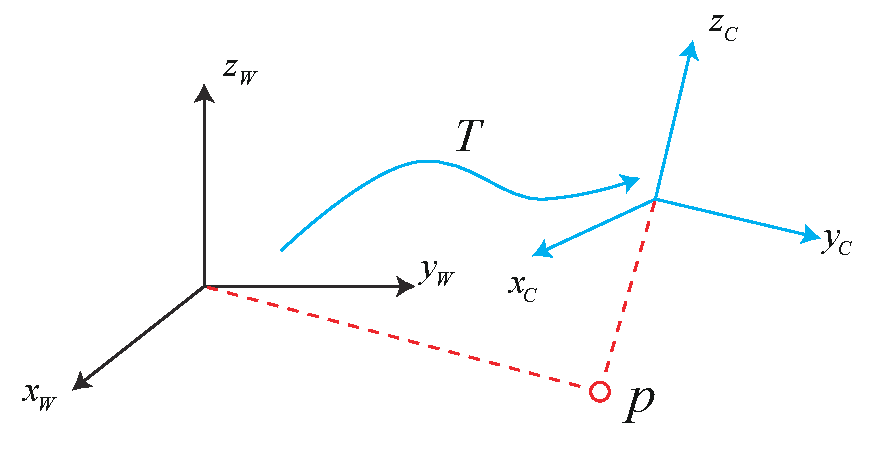
\includegraphics[width=0.7\textwidth]{chapter03/rigidMotion/axisTransform.pdf}
	\caption {Coordinate transformation. For the same vector $ \bm{} the p- $ , it coordinates in the world coordinate system $ \bm{} _w the p- $ and coordinate in the camera coordinate system $ \bm{} _c the p- $ is different. This transformation relationship is described by the transformation matrix $ \bm{T} $ . }
	\label{fig:axisTransform}
\end{figure}

Intuitively, the motion between two coordinate systems consists of a rotation plus a translation called \textbf {rigid body motion}. Camera movement is a rigid body movement. During the rigid body motion, the length and angle of the same vector in each coordinate system will not change. Imagine you throw your phone into the air and \footnote {Please don't put it into practice before it falls to the ground . }, there may only be differences in spatial position and posture, and its own length, angle of each face, etc. will not change. The phone will not be squashed like an eraser for a while, and will be stretched for a while. At this point, we say that the phone coordinate system is between the world coordinates, which is a difference of \textbf {Euclidean Transform}.

The Euclidean transformation consists of rotation and translation. We first consider rotation. Let a unit of orthogonal base $ ( \bm {e}_ 1 , \bm {e}_ 2 , \bm {e}_ 3 ) $ after a rotation becomes $ ( \bm {e}_ 1 ' , \bm {e}_ 2 ', \bm {e}_ 3 ') $ . Then, for the same vector $ \bm {a} $ (the vector does not move with the rotation of the coordinate system), its coordinates in two coordinate systems are $ [a_ 1 , a_ 2 , a_ 3 ] ^ \mathrm {T} $ and $[a'_ 1 , a'_ 2 , a'_ 3 ]^ \mathrm {T} $ . Because the vector itself has not changed, according to the definition of coordinates, there are:

\begin{equation}
\left[ \bm{e}_1,\bm{e}_2,\bm{e}_3 \right]\left[ \begin{array}{l}
{a_1}\\
{a_2}\\
{a_3}
\end{array} \right] = \left[ \bm{e}_1', \bm{e}_2', \bm{e}_3' \right]\left[ \begin{array}{l}
a'_1\\
a'_2\\
a'_3
\end{array} \right].
\end{equation}

To describe the relationship between the two coordinates, we multiply the left and right sides of the above equation by $ \left [ \begin {array}{l}
\bm{e}_1^\mathrm{T}\\
\bm{e}_2^\mathrm{T}\\
\bm{e}_3^\mathrm{T}
\end {array} \right ] $ , then the coefficient on the left becomes the identity matrix, so:
%\clearpage
\begin{equation}
\left[ \begin{array}{l}
{a_1}\\
{a_2}\\
{a_3}
\end{array}\right]=\left[{\begin{array}{*{20}{c}}    
	{\bm{e}_1^\mathrm{T}\bm{e}_1'} & {\bm{e}_1^\mathrm{T}\bm{e}_2'} & {\bm{e}_1^\mathrm{T}\bm{e}_3'}\\
	{\bm{e}_2^\mathrm{T}\bm{e}_1'} & {\bm{e}_2^\mathrm{T}\bm{e}_2'} & {\bm{e}_2^\mathrm{T}\bm{e}_3'}\\
	{\bm{e}_3^\mathrm{T}\bm{e}_1'} & {\bm{e}_3^\mathrm{T}\bm{e}_2'} & {\bm{e}_3^\mathrm{T}\bm{e}_3'}
	\end{array}} \right]\left[ \begin{array}{l}
a_1'\\
a_2'\\
a_3'
\end{array} \right] \buildrel \Delta \over = \bm{R} \bm{a}'.
\end{equation}
We take the intermediate matrix out and define it as a matrix $ \bm{R} $ . This matrix consists of the inner product between the two sets of bases, characterizing the coordinate transformation relationship of the same vector before and after the rotation. As long as the rotation is the same, then this matrix is the same. It can be said that the matrix $ \bm{R} $ describes the rotation itself. So called \textbf{rotation matrix} (Rotation matrix). At the same time, the components of the matrix are the inner product of the two coordinate system bases. Since the length of the base vector is 1, it is actually the cosine of the angle between the base vectors. So this matrix is also called \textbf{Direction Cosine Matrix}. We will call it a rotation matrix in the following.

The rotation matrix has some special properties. In fact, it is an orthogonal matrix with a determinant of 1 \footnote{orthogonal matrix that is inversely transposed by itself. The orthogonality of the rotation matrix can be derived directly from the definition. } \footnote{The determinant is 1 is artificially defined. In fact, only its determinant is $ \pm  1 $ , but the determinant is $ - 1 $ is called R rotation, that is, one rotation plus one reflection. }. Conversely, an orthogonal matrix with a determinant of 1 is also a rotation matrix. So, you can define a collection of $ n $ dimensional rotation matrices as follows:
\begin{equation}
\mathrm{SO}(n) = \{ \bm{R} \in \mathbb{R}^{n \times n} | \bm{R R}^\mathrm{T} = \bm{I}, \mathrm{det} (\bm{R})=1 \}.
\end{equation}

$ \mathrm {SO}(n) $ isthe meaningof \textbf {Special Orthogonal Group}. We leave the contents of the "group" to the next lecture. This collection consists ofa rotation matrix of $ n $ dimensional space, in particular, $ \mathrm {SO}( 3 ) $ refers to the rotation of the three-dimensional space. By rotating the matrix, we can talk directly about the rotation transformation between the two coordinate systems without having to start from the base.

Since the rotation matrix is an orthogonal matrix, its inverse (ie, transpose) describes an opposite rotation. According to the above definition, there are:
\begin{equation}
\bm{a} '= \bm{R}^{-1} \bm{a} = \bm{R}^ \mathrm{T} \bm{a}.
\end{equation}
Obviously $ \bm{R}^\mathrm{T} $ portrays an opposite rotation.

In the Euclidean transformation, there is translation in addition to rotation. Consider the vector $ \bm{a} $ in the world coordinate system , after a rotation ( depicted by $ \bm{R} $ ) and a translation of $ \bm{t} $ , you get $ \bm{a}' $ , then put the rotation and translation together, there are:
\begin{equation}
\label{eq:RT}
\ bm {a} '= \ bm {R} \ bm {a} + \ bm {t}.
\end{equation}
Where $ \bm{t} $ is called a translation vector. Compared to rotation, the translation part simply adds the translation vector to the coordinates after the rotation, which is very simple. By the above formula, we completely describe the coordinate transformation relationship of an Euclidean space using a rotation matrix $ \bm{R} $ and a translation vector $ \bm{t} $ . In practice, we will define the coordinate system 1, coordinate system 2, then the vector $ \bm{a} $ under the two coordinates is $ \bm{a}_1 , \bm{a}_2 $ , they are The relationship between the two, in accordance with the complete writing, should be:
\begin{equation}
\ bm{a}_1 = \bm{R}_{12} \bm{a}_2 + \bm{t}_{12}.
\end{equation}
Here $ \bm{R}_{12} $ means "transform the vector of coordinate system 2 into coordinate system 1". Since the vector is multiplied to the right of this matrix, its subscript is \textbf{read from right to left}. This is also the customary way of writing this book. Coordinate transformations are easy to confuse, especially if multiple coordinate systems exist. Similarly, if we want to express "rotation matrix from 1 to 2", we write it as $ \bm{R}_{21} $ . The reader must be clear about the notation here, because different books have different writing methods, some will be recorded as the top left/subscript, and the text will be written on the right side.

About panning $ \bm {t}_{12} $ , it actually corresponds to the coordinate system 1 origin pointing to the coordinate system 2 origin vector, \textbf{ coordinates taken under coordinate system}, so I suggest readers to put it It is written as "a vector from 1 to 2." But the reverse $ \bm {t}_{21} $ , which is a vector from 2 to 1 \textbf{coordinates in coordinate system 2}, is not equal to $ - \bm{t}_{12} $ , but related to the rotation of the two systems \footnote{although from the vector level, they are indeed inverse relations, but the coordinates of the two vectors are not opposite. Can you think about why this is? }. Therefore, when beginners ask the question "Where is my coordinates?", we need to clearly explain the meaning of this sentence. Here "my coordinates" actually refers to the vector from the world coordinate system pointing to the origin of the coordinate system of the world, and the coordinates obtained in the world coordinate system. Corresponding to the mathematical symbol, it should be the value of $ \bm{t}_{WC} $ . For the same reason, it is not $ - \bm {t}_{CW} $ .

